\documentclass[review]{elsarticle}

\usepackage{lineno,hyperref}
\modulolinenumbers[5]
\usepackage{amsfonts}
\usepackage{algorithmicx}
\usepackage[ruled]{algorithm}
\usepackage{algpseudocode}
\usepackage{algpascal}
\usepackage{algc}
\usepackage{multirow}
\usepackage{amsmath}
\alglanguage{pseudocode}
\usepackage{subfig}% http://ctan.org/pkg/subfig
\usepackage{booktabs}% http://ctan.org/pkg/booktabs
\journal{Computer Speech and Language}

\usepackage{multirow}
\usepackage{multicol}

%%%%%%%%%%%%%%%%%%%%%%%
%% Elsevier bibliography styles
%%%%%%%%%%%%%%%%%%%%%%%
%% To change the style, put a % in front of the second line of the current style and
%% remove the % from the second line of the style you would like to use.
%%%%%%%%%%%%%%%%%%%%%%%

%% Numbered
%\bibliographystyle{model1-num-names}

%% Numbered without titles
%\bibliographystyle{model1a-num-names}

%% Harvard
%\bibliographystyle{model2-names.bst}\biboptions{authoryear}

%% Vancouver numbered
%\usepackage{numcompress}\bibliographystyle{model3-num-names}

%% Vancouver name/year
\usepackage{numcompress}\bibliographystyle{model4-names}\biboptions{authoryear}

%% APA style
%\bibliographystyle{model4-names}\biboptions{authoryear}

%% AMA style
%\usepackage{numcompress}\bibliographystyle{model6-num-names}

%% `Elsevier LaTeX' style
%bibliographystyle{elsarticle-num}
%%%%%%%%%%%%%%%%%%%%%%%
\usepackage{url}
\def\UrlBreaks{\do\/\do-}
\begin{document}

\begin{frontmatter}

\title{Sequential Routing Framework: \\Fully Capsule Network-based Speech Recognition}

%% Group authors per affiliation:
\author[address_snu,address_sec]{Kyungmin Lee}
\author[address_snu]{Hyunwhan Joe}
\author[address_sec]{Hyeontaek Lim}
\author[address_sec]{Kwangyoun Kim}
\author[address_sec]{Sungsoo Kim}
\author[address_sec]{Chang Woo Han}
\author[address_snu]{Hong-Gee Kim\corref{corresponding}}

\cortext[corresponding]{Corresponding author}
\ead{hgkim@snu.ac.kr}
\address[address_snu]{Biomedical Knowledge Engineering Laboratory, Seoul National University, Seoul, 08826, Republic of Korea}
\address[address_sec]{Samsung Research, 56, Seongchon-gil, Seocho-gu, Seoul, 06765, Republic of Korea}

\begin{abstract}
Capsule networks (CapsNets) have recently gotten attention as alternatives for convolutional neural networks (CNNs) with their greater hierarchical representation capabilities.
In this paper, we introduce the sequential routing framework (SRF) which we believe is the first method to adapt a CapsNet-only structure to sequence-to-sequence recognition.
In SRF, input sequences are capsulized then sliced by the window size.
Each sliced window is classified to a label at the corresponding time through iterative routing mechanisms.
Afterwards, training losses are computed using connectionist temporal classification (CTC).
During routing, two kinds of information, learnable weights and iteration outputs are shared across the slices.
By sharing the information, the required parameter numbers can be controlled by the given window size regardless of the length of sequences.
Moreover, the method can minimize decoding speed degradation caused by the routing iterations since it can operate in a non-iterative manner at inference time without dropping accuracy.
We empirically proved the validity of our method by performing phoneme sequence recognition tasks on the TIMIT corpus.
The proposed method attains an 82.6\% phoneme recognition rate.
It is 0.8\% more accurate than that of CNN-based CTC networks and on par with that of recurrent neural network transducers (RNN-Ts).
Even more, the method requires less than half the parameters compared to the two architectures.
\end{abstract}

\begin{keyword}
Capsule network\sep Automatic speech recognition\sep Sequence-to-sequence\sep Connectionist temporal classification
\end{keyword}

\end{frontmatter}

\linenumbers

\section{Introduction}
Capsule networks (CapsNets) \citep{DBLP:conf/icann/HintonKW11, DBLP:conf/nips/SabourFH17, DBLP:conf/iclr/HintonSF18} are a kind of neural network that represents a specific entity type by a group of neurons, which are referred to as capsules, instead of a single neuron represented in a scalar.
The initial motivation of CapsNets was to abstract information more explicitly by adapting an unsupervised clustering method called routing-by-agreement to neural networks.
By introducing the new representation units, the routing mechanism can be performed between adjacent capsules during neural network training.
Capsules can represent not only the existence of the entity types but also entity instantiation parameters such as textures, angles, colors, and so on, thus CapsNets can be regarded as inverse rendering architectures.
They have received notable attention as promising alternatives to convolutional neural networks (CNNs).
Particularly, this is because the pooling layers in CNNs filter information within each patch from lower to higher layers based on fixed operations such as maximum or average, unlike the adaptive mechanism i.e. routing mechanisms in CapsNets.
CapsNets have shown higher accuracy in image classification on MNIST \citep{lecun-mnisthandwrittendigit-2010} and Canadian Institute For Advanced Research (CiFAR) 10 \citep{Krizhevsky09learningmultiple} than CNNs \citep{DBLP:conf/nips/HahnPK19, Malmgren1314210}.
Previously, research on CapsNets have mostly focused on improving the performance of routing methods \citep{Malmgren1314210, DBLP:conf/iclr/Wang018} on smaller datasets.
Recently, research has been focused more on modifying the routing methods to fit more practical problems such as scaling the routing methods itself \citep{DBLP:conf/iclr/TsaiSGS20} or by combining them with other architectures \citep{DBLP:conf/icann/HePLHZ19, 8852016, wang-2019-towards}.
There have also been attempts to apply CapsNet to various fields beyond image classification such as user intent detection \citep{DBLP:conf/emnlp/XiaZYCY18, DBLP:conf/acl/ZhangLDFY19}, self-driving \citep{DBLP:journals/tjs/KimC19},
sound event detection \citep{DBLP:conf/eusipco/Iqbal0KW18}, speech command classification \citep{DBLP:conf/interspeech/BaeK18} and speech emotion recognition \citep{DBLP:conf/icassp/WuLCLYDMHWLM19}.

A sequence to sequence (seq2seq) learning is an approach to learn mappings between input and output sequences and the the learning is successfully implemented by neural models \citep{DBLP:conf/nips/SutskeverVL14}.
It is one of the most popular methods in a wide range of fields such as automatic speech recognition (ASR) \citep{DBLP:conf/icassp/ChanJLV16, DBLP:conf/icassp/HeSPMAZRKWPLBSL19, DBLP:conf/asru/KimJLHKLGPKJLYK19, DBLP:conf/asru/MoritzHR19}, machine translation (MT) \citep{DBLP:journals/corr/BahdanauCB14, DBLP:conf/interspeech/JiaWBMJCW19}, natural language processing (NLP) \citep{DBLP:conf/ijcai/YinJLSLL16}, etc.
Connectionist temporal classification (CTC) \citep{DBLP:conf/icml/GravesFGS06} is a popular loss function in seq2seq problems since the method can compute a conditional probability between a single reference and multiple possible paths of a network output vector sequence.
As CTC started to be applied to ASR tasks, it became possible to learn the alignment between speech signal sequences and label sequences directly unlike the conventional Hidden Markov Model (HMM)-based methods \citep{18626} that need separately aligned intermediate representations.
Recurrent neural network transducers (RNN-Ts) \citep{DBLP:conf/icassp/GravesMH13} have expanded CTC by introducing an additional axis to represent linguistic information. They are now one of the most pervaded methods in the commercial ASR systems \citep{DBLP:conf/icassp/HeSPMAZRKWPLBSL19}.
Recently, CTC networks are also used as a form of joint training \citep{DBLP:conf/asru/KimJLHKLGPKJLYK19, DBLP:conf/asru/MoritzHR19} with cross-entropy based networks to help encoders learn better alignments when training attention-based encoder-decoder models.

In seq2seq problems, long short term memory (LSTM) \citep{DBLP:journals/neco/HochreiterS97} is one of the most common approaches.
LSTMs are a kind of recurrent neural networks (RNNs) and have better sequence encoding capabilities than vanilla RNNs since they can learn more explicitly how to filter contextual information with cell states and gating mechanisms implemented as non-linear activation functions.
CTC networks were first built based on LSTMs \citep{DBLP:conf/icml/GravesFGS06} and they have shown competitive performance compared to traditional ASR methods.
In particular, bidirectional LSTM (BLSTM)-based CTC networks have shown the most accurate recognition rate among the early implementations \citep{DBLP:conf/icassp/GravesMH13}.
In order to relieve computational burden and avoid the vanishing and exploding gradient problem of LSTMs, a CNNs-based CTC network \citep{DBLP:conf/interspeech/ZhangPBZLBC16} has been proposed as an alternative.
CNNs encode the input feature sequences by filtering the context information with their own mechanisms which convolve the sequences with multiple filters to detect specific shapes.
They then down-sample the convolved sequences with pooling methods as explained earlier in this section.
Through this hierarchical structure, they can encode spatial relations wider than each filter size with deeper convolutional layers.
Recently, Transformers which are self-attention-based neural architectures \citep{DBLP:conf/nips/VaswaniSPUJGKP17}, have been in the spotlight as another alternative to the recurrent models.
Transformers encode sequences by filtering with attention maps which indicate within-sequence similarities calculated with scaled dot-products.
Although Transformers do not have an appropriate structure for streaming decoding since they need the whole context to compute the attention map, there have been recent attempts to apply them to streaming decoding \citep{9054476}.
With their own context filtering mechanisms, the two alternative methods have shown similar or better accuracy compared to LSTMs in ASR related fields \citep{DBLP:conf/interspeech/ZhangPBZLBC16, 8462506, DBLP:journals/corr/abs-1812-06864, 9054476} while requiring less computations and have suitable structures for parallelization.
In particular, the CNN-based CTC networks \citep{DBLP:conf/interspeech/ZhangPBZLBC16} have shown 0.2\% more accurate phoneme recognition rate (PRR) with 63.2\% of parameters compared to the BLSTM-based architecture while maintaining online decoding capabilities.
The input feature sequences can be regarded as two dimensional images which having time length as width and the feature dimension as height.
In this perspective, we hypothesized that CapsNets can potentially have richer representation capabilities than CNNs also in seq2seq problems for the same reasons mentioned earlier in this section.
Research on CapsNets have mostly focused on classification tasks with fixed input sizes as alternatives for CNNs.
Although there have been attempts to apply CapsNets to seq2seq tasks in combination with other models \citep{8852016, wang-2019-towards}, the utilization of CapsNets could be maximized more.
There are several hurdles in applying existing CapsNet-only architectures to seq2seq problems without modification.
This is because routing from the variable-length capsule inputs to the sequential combinations of labels is infeasible in the perspectives of both computation and the required parameter amount.
Furthermore, ASR systems which are one of the most common seq2seq applications essentially require real-time processing, which can be hampered by the computationally expensive iterative routing mechanisms. 

In this paper, we introduce the sequential routing framework (SRF) which is a novel method to build up CTC networks based on a CapsNet-only architecture.
SRF is applicable to iterative routing-by-agreement methods \citep{DBLP:conf/nips/SabourFH17, DBLP:conf/iclr/HintonSF18} which update the routing coefficients of the current iteration using the outputs of the previous iteration in an expectation and maximization manner.
In order to validate our proposed method, we performed phoneme sequence recognition by applying Dynamic routing (DR) \citep{DBLP:conf/nips/SabourFH17} to the framework because it has shown competitive performance~\citep{DBLP:conf/nips/HahnPK19, Malmgren1314210}.
To train SRF models, the input feature sequences for the framework are first converted to three-dimensional sequences through convolutional and linear projection layers.
The encoded sequences are sliced by time windows and multiple routing iterations are performed for each slice to classify the corresponding label.
Afterwards, the training loss is calculated using CTC.
The framework achieved competitive accuracy while minimizing decoding speed degradation and required parameters by temporally sharing two types of information during routing.
In this paper, what we mean by ``temporally sharing" is to share information across the time slices.
First, the learnable variables for computing the path representations from lower to higher levels are shared so that only the fixed size of parameters, according to the given window size, is required.
In addition to the weight sharing, the capsule clustering information is also conveyed to the next time slice by initializing routing coefficients of the current slice based on the previous routing results.
As a result, iteration is not required during inference meanwhile the routing coefficients can have an effect similar to be updated by the number of times corresponding to each window time slice.

A clear contribution of this study is that, to the best of our knowledge, SRF is the first CapsNets only architecture for the seq2seq recognition problem. 
The proposed method achieved competitive performance on the speech recognition task in three aspects that are accuracy, decoding speed, and parameter numbers by temporally sharing learnable weights and clustering information.

\section{Preliminaries}
\subsection{CTC Network}
A CTC network \citep{DBLP:conf/icml/GravesFGS06} is defined as a continuous map \(\mathcal{N}_\theta: (\mathbb{R}^F)^T \mapsto (\mathbb{R}^{V})^T\) from an \(F\) dimensional input sequence \(x\) of length \(T\) to the same length sequence \(\hat{y}\) of \(V\) dimensional probability vectors with parameters \(\theta\).
\(V\) is the cardinality of an expanded label set \(\mathbb{L}'\) consisting of the union between the label symbol set \(\mathbb{L}\) and the blank symbol set, \(\mathbb{L} \cup \{<\)blank\(>\}\).
This network contains a softmax layer at the top of it in order to convert logits to valid probability distributions.
The softmax layer for a given vector \(Z \in \mathbb{R}^D\) is computed as follows:
\begin{equation}
\text{softmax}(Z)_i = {{\exp(z_i)} \over {\sum^D_{j=1} \exp(z_{j})}}, \text{for } i=1,...,D
\label{eq:softmax}
\end{equation}
, where \(z_i\) is the \(i\)-th element of \(Z\).
CTC computes a conditional probability of a label sequence \(y \in \mathbb{L} ^{\leq T}\) for a given input sequence \(x\) by summing up every conditional probability of possible paths \(\pi\), i.e. \(p(y|x) = \sum_{\pi \in \mathcal{B}^{-1}(y)} p(\pi|x)\).
The possible paths are computed using an inverse of a map \(\mathcal{B}: \mathbb{L}^{\prime T} \mapsto \mathbb{L}^{\leq T}\) from an expanded label sequence \(y^\prime\) to \(y\).
\(\mathcal{B}\) performs many-to-one mappings by simply removing repeating and blank symbols from the given paths.
For example, \(\mathcal{B}\)(``cc-aaa-tt") = \(\mathcal{B}\)(``-cc-aattt") = ``cat", where ``-" indicates a blank symbol.
It allows CTC networks to learn alignments solely from the input and output sequence pairs.
A conditional probability of each possible path is computed as \(p(\pi|x)=\prod_{t=1}^T p(y^{\prime t}_\pi |x^t)\), where \(y^{\prime t}_\pi\) is an expanded label symbol in a path \(\pi\) at time \(t\) and \(x^t\) is the \(t\)-th feature vector of \(x\).
An objective function is defined to compute a negative summation of log probabilities of all the possible paths corresponding to the given labeling and CTC networks are trained to minimize it.
The gradient of the objective function can be computed with respect to \(\hat{y}\) with any kind of gradient-based optimization techniques.
To derive the gradient more efficiently, the CTC forward-backward algorithm, which is a kind of dynamic programming, is applied during training.

\subsection{Capsule Network}
The main structural difference of CapsNets with other neural architectures is that they use a group of neurons as an element of representation rather than a single neuron \citep{DBLP:conf/icann/HintonKW11}.
The group of neurons is referred to as a capsule and it consists of an activation scalar and a group of instantiation parameters.
For a certain entity type, the former indicates an existence probability while the latter represents characteristics such as deformations, poses, and textures in the form of a vector or matrix.
Thus, encoding image data through CapsNets can be seen as a mechanism of inverse renderings which converts input data to their instantiation parameters.
The activations can be computed either from the instantiation parameters~\citep{DBLP:conf/nips/SabourFH17} or from additional neural layers~\citep{DBLP:conf/iclr/HintonSF18}, according to the routing mechanisms.
With the two representations, CapsNets can potentially~\citep{NIPS2018_8100} represent invariance of the existence probabilities and also equivariance of the properties of the entity type.
The input and output of capsule layers are the group of capsules which have a three-dimensional structure.
Accordingly, a capsule group is composed of a pair of an instantiation parameter vector group and its corresponding activation scalar group.
In this paper, for the sake of brevity, we describe the structure of an instantiation vector group in a capsule group as the structure of the capsule group because the structure of the activation scalar group can be derived by just removing the depth of the vector group structure.
The product of the width and height of a capsule group indicates the number of capsules in the group and their depth represents the dimension of the instantiation parameter vectors.
The capsule groups in the lowest, the highest, and in-between levels of CapsNets are called as primary, class, and convolutional capsule groups respectively.
The width of class capsule groups is one and its height is equal to the number of labels for classification tasks.
In order to compare the class capsule group with the given label, each instantiation vector of the group is flatten to an activation i.e. the final output structure of a CapsNet is converted to the same as that of a conventional neural network.
Thus any loss methods used for other neural networks are applicable for CapsNets without modification.

One of the key abilities of neural networks is to abstract the information in input data to higher concepts layer by layer, in order to make them a suitable representation for the purpose of training.
We can assume that this hierarchical conceptualization can be seen as a tree-like structure made of multiple part-whole relationships.
In order to use this assumption more explicitly to train models, CapsNets introduce the routing-by-agreement method which is a kind of unsupervised clustering algorithm.
The method routes information from lower to higher levels based on the agreements of capsules.
In this perspective, the routing mechanism can be thought of as an adaptive layer-wise filtering method compared to both static filtering such as striding or pooling of CNNs and sequence-wise filtering such as the gates of LSTMs or self-attentions of Transformers.
The one key procedural difference is that routing-by-agreement is a non-gradient based learning algorithm.
Research related to CapsNets have mainly focused on iterative routing methods which update their clustering mechanisms based on the outputs of previous iterations \citep{DBLP:conf/nips/SabourFH17, DBLP:conf/iclr/HintonSF18}.
Recently in order to reduce their computational burdens, non-iterative \citep{DBLP:conf/nips/HahnPK19} or parallelized \citep{DBLP:conf/iclr/TsaiSGS20} methods have also been introduced.

\subsubsection{Dynamic Routing} % Dynamic Routing 정의, 동작 방법(알고리즘 포함)
DR \citep{DBLP:conf/nips/SabourFH17} is a kind of iterative routing-by-agreement method that controls information flow from lower to higher levels based on the capsule similarities between the adjacent capsule groups in a non-parametric manner.
It is one of the most widely used implementation of CapsNets because of its competitive accuracy and intuitive mechanisms compared to more recent architectures  \citep{DBLP:conf/nips/HahnPK19, Malmgren1314210}.
In DR, activation scalars of capsules are defined by the lengths of the instantiation parameter vectors so that they need to be normalized to have bounded lengths within the range from zero to one.
In order to normalize them, a nonlinear function, which is referred to as a squash function, is defined as follows:
\begin{equation}
\text{squash}(s) = {{||s||^2} \over{1+||s||^2}} {{s}\over{||s||}}
\label{eq:squash}
\end{equation}
, where $s$ is a unnormalized instantiation parameter vector.
This function also has a role to make the output activations more discriminative by pushing most of the values to around zero or one.
The $s$ for the $j$-th capsule of the output capsule group is computed as $s_j = \sum^{l_N}_i c_{ij} \hat{u}_{j|i}$, that is the summation of the prediction vector $\hat{u}_{j|i}$ from the $i$-th capsule in the lower level to the $j$-th capsule in the higher level weighted with corresponding coupling coefficients $c$.
The coefficients are normalized values through the softmax function described in Eq.~\ref{eq:softmax} from the routing coefficients r, which is updated by a routing method.
$\hat{u}_{j|i}$ is calculated as the multiplication of an instantiation parameter vector $u_i$, which is the $i$-th capsule in an input capsule group, and a learnable weight matrix $W_{ij}$.
Thus the required number of $W$ for each routing mechanism is the product of the capsule numbers of input and output capsule groups and each $W_{ij}$ has the shape of the input capsule depth times the output capsule depth.
The primary capsules are calculated from input data through multiple convolutional layers activated with rectified linear unit (ReLU) functions.

In the routing algorithm, $r$ is initialized uniformly, then it is iteratively updated to maximize the agreements between $\hat{u}_{j|i}$ and the output vector $o_j$ by accumulating the values of their products.
In order to allow for multiple digits, a separate margin loss between labels and the activations of the final output vectors is calculated as a prediction error.
Reconstruction errors are calculated as the mean squared errors between the original signals and the reconstructed signals generated from the output capsule corresponding to the target label through additional feed forward layers.
A total loss for training is computed by adding a reconstruction error to the prediction error as a regularization term.

\section{Sequential Routing Framework}
\begin{figure*}[ht!]
  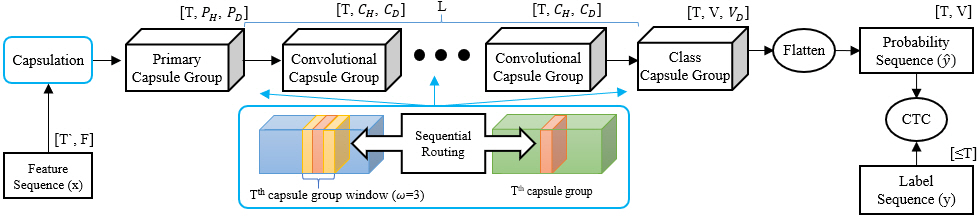
\includegraphics[trim={0 0cm 0 0cm}, clip, width=1.0 \linewidth]{01_overview.jpg}
  \caption{An overview of the sequential routing framework (SRF)}
  \label{fig:diagram}
\end{figure*}
SRF is an iterative routing framework for sequence data and it is defined as a modified version of CTC networks with parameter $\psi$, $\mathcal{S}_\psi: (\mathbb{R}^{F^\prime})^{T^\prime} \mapsto (\mathbb{R}^V)^T$, from a real valued feature sequence $x$ having a length $T^\prime$ and a feature dimension $F^\prime$ to a $V$ dimensional probability vector sequence $\hat{y}$ of a width $T$ as shown in Fig.~\ref{fig:diagram}.
The shapes of an input or output sequence and each capsule group are written above the boxes in the diagram.
A two-dimensional input feature sequence $x$ is transformed into a primary capsule group, whose width, height and depth are $T$, $P_H$ and $P_D$ respectively, through a capsulation block.
Afterwards, the primary capsule group is fed into the lowest capsule layer, then encoded to a convolutional capsule group, whose width, height and depth are $T$, $C_H$, and $C_D$ respectively.
For the sake of brevity, we describe all the convolutional capsule groups have the same shape.
The output of the $L$-th capsule layers, i.e. a class capsule group, has $T$, $V$, and $V_D$ as width, height and depth respectively.
The capsule group is flattened to an activation vector sequence $\hat{y}$ which is a sequence of probability vectors where each element indicates a probability of observing a corresponding label symbol.
If $L$ is set to one, the lowest capsule layer directly outputs class capsule groups.
Finally, a negative log probability is computed using CTC between $\hat{y}$ and a given label sequence $y$ as a loss for training the neural network.

\subsection{Capsulation}
\begin{figure}[hbt!]
  \centering
  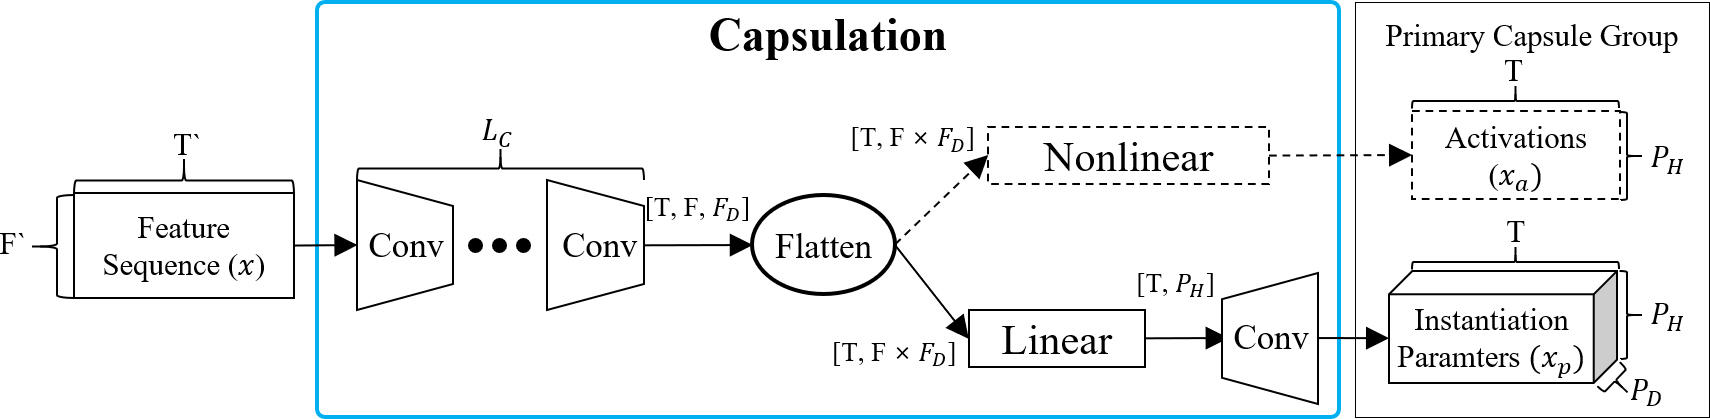
\includegraphics[trim={0 0cm 0 0cm}, clip, width=1.0\linewidth]{02_capsulation.jpg}
  \caption{A capsulation block}
  \label{fig:capsulation}
\end{figure}
Capsulation is a neural layer block that converts from $x$ to a group of primary capsules which consists of two subgroups as shown in the Fig.~\ref{fig:capsulation}.
One group is an activation group with dimensions of width $T$ and height $P_H$ and 
the other is an instantiation parameter group with width $T$, height $P_H$ and dimension $P_D$. 
The layers to compute the group of activations are optional structures depending on the routing mechanism.
A feature sequence $x$ is encoded into three-dimensional representation with width $T$, height $F$ and depth $F_D$ through $L_C$ two-dimensional convolutional layers, where $T \leq T^\prime$ and $F \leq F^\prime$.
We employed maxout~\citep{DBLP:journals/corr/abs-1302-4389} as activation functions of the convolutional layers because of their competitive accuracy in ASR systems~\citep{DBLP:conf/interspeech/ZhangPBZLBC16}.
Thus, the \(l_c\)-th convolutional layer in the first sub-block is defined as follows:
\begin{equation}
x_{l_c}=\max_{n_c \in [1, N_C]} \text{Dropout}_{n_c}([W_{l_c, n_c, f_d}*x_{l_c-1}]_{f_d=1}^{F_D}, \alpha_d)\text{, }l_c \in [1, L_C]
\label{eq:maxout}
\end{equation}
, where $*$ is a convolutional operator, $N_C$ is the number of convolutional operations in a layer and $\alpha_d$ is the dropout rate. $W_{l_c, n_c, f_d}$ indicates a convolution weight matrix for the $f_d$-th channel of the $n_c$-th convolutional operation in the $l_c$-th layer.
The $0$-th $x$ is an input sequence, i.e. $x_0 \in (\mathbb{R}^{F^\prime})^{T^\prime}$.
For all the cases, we set $N_C$ and $\alpha_d$ to 2 and 0.2 respectively.
Subsequently, the output sequence is flattened to $x^\prime_{L_C}$ by simply reshaping it to width $T$ and height $F \times F_d$, then it is fed into two kinds of layer blocks.
One of them is projected to a normalized vector sequence, i.e. an activation group $x_a$, with width $T$ and height $P_H$, through a nonlinear layer as follows:
\begin{equation}
x_a=\sigma(W_{a} \times x^\prime_{L_C})
\label{eq:nonlinear}
\end{equation}
, where \(W_a\) is a learnable weight matrix and \(\sigma\) is a nonlinear function for normalizing the values.
The other is projected to another representation having the same shape with the activation group as follows:
\begin{equation}
x_p^\prime=W_{p} \times x^\prime_{L_C}
\label{eq:linear}
\end{equation}
, where \(W_p\) is a learnable weight matrix.
Afterwards, it is converted to a group of instantiation parameters \(x_p\) by expanding their channel dimensions into \(P_D\) through a two-dimensional convolutional layer activated with the maxout function as follows:
\begin{equation}
x_p=\max_{n_c\in[1, N_C]}\text{Dropout}_{n_c}([W_{n_c, p_d} * x_p^\prime]_{p_d=1}^{P_D}, \alpha_d)
\label{eq:maxout2}
\end{equation}
, where $W_{p_d}$ indicate a convolutional weight matrix for the $p_d$-th output channel of the $n_c$-th convolutional operation.
We set $N_C$ and $\alpha_d$ identically for every layer activated with maxout in order to reduce the number of hyperparameters.

\subsection{Routing-by-agreement for sequence to sequence learning}
In SRF, each subgroup of a capsule group $\{x_a, x_p\}$ is sliced by $t$, i.e. $x^t=\{x_a^t, x_p^t\}$. The routing mechanism which we will refer to as sequential routing is performed for the each slice.
In order to expand the size of a receptive field on a primary capsule group, sequential routing is performed between window slices, which consist of $\omega$ slices of the lower level, and single slices of the higher level.
The bottom box in Fig.~\ref{fig:diagram} describes an example of sequential routing between the $t$-th window slice ($\omega = 3$) in the lower level and the $t$-th single slice in the higher level.
In this study, we set the stride of the sliding window to one in all the cases and the both side of window contexts beyond the sequence boundaries are padded as zero so that the routing is performed $T$ times for a primary capsule group having width $T$.
The width of the receptive field on a primary capsule group is computed as $\omega + (L-1) \times (\omega - 1)$ for each slice of the output of the \(L\)-th capsule layer.
Accordingly, online decoding is allowed with a time delay corresponding to \(L \times \omega_R\), where \(\omega_R\) is the right context size of the window.
In each capsule layer, the prediction vector \(\hat{u}_{j|i}\) is calculated per each \(t\) through a linear transformation consisting of a learnable weight matrix \(W_{ij}\) as follows:
\begin{equation}
\hat{u}_{j|i}^t = W_{ij} \times x_{p_i}^t, i \in [1, \omega \times I_H], j \in [1, O_H]
\label{eq:uhat}
\end{equation}
, where $I_H$ and $O_H$ are heights of input and output capsule groups respectively and each $W_{ij}$ has the shape of the product of dimensions of input and output capsule groups.
Consequently, the number of parameters to perform the routing method in each capsule layer is controlled by the given three kinds of hyper parameters, that are the height and depth of capsule groups and $\omega$, regardless of the input sequence length since the parameters are temporally shared across all $t$.

\begin{figure}[ht]
\centering
\subfloat[original][Original routing]{
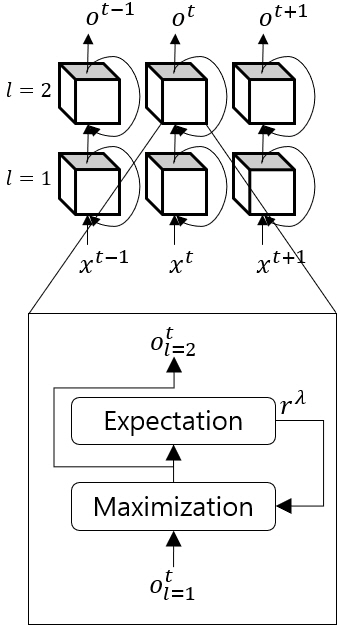
\includegraphics[width=0.35\linewidth]{03a_routing_original.jpg}
\label{fig:diagram_3_or}
}
\qquad\qquad
\subfloat[sequential][Sequential routing]{
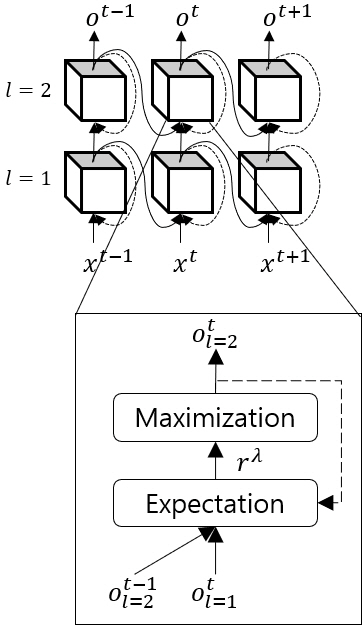
\includegraphics[width=0.37\linewidth]{03b_routing_sequential.jpg}
\label{fig:diagram_3_sr}
}
\caption[]{Schematic diagrams of the two versions of iterative routing procedures ($L=2$, $\omega=1$, $\lambda \in [1, \Lambda]$).}
\label{fig:diagram3}
\end{figure}

We have an assumption that consecutive slices in sequence data have similar properties.
Based on that, we designed an iterative routing mechanism which initializes routing coefficients of the $t$-th iteration based on the $(t-1)$-th iteration outputs.
Fig.~\ref{fig:diagram3} is a schematic diagram of the two different iterative routing mechanisms of $L=2$ and $\omega=1$ for three consecutive window slices.
In this figure, the three dimensional block represents the routing procedures, $\lambda$ is an iteration index in the range between 1 and the given iteration number $\Lambda$, and the solid and dashed arrows describe the required and optional flows to update routing coefficients $r$ respectively.
In the original version of routing, $r$ is initialized uniformly, then updated within each $t$ iteratively as in Fig.~\ref{fig:diagram_3_or} in the order of a maximization and an expectation stages.
The expectation stage means to update $r$ to improve the agreements between adjacent capsule groups and the updated coefficients are applied in the maximization stage.
The proposed sequential routing method has two procedural differences from the original version as described in Fig.~\ref{fig:diagram_3_sr}.
First, $r$ is initialized based on the agreements between the previous routing outputs $o_{l}^{t-1}$ and the current routing inputs $o_{l-1}^{t}$ thus $r$ is uniformly initialized only at $t=1$.
The second procedural difference is the sub-procedure order of the routing mechanism which expects the initial $r$ before the first maximization stage.
These two modifications have a similar effect of updating $r$ for $(t-1)$ times to compute the $t$-th output $o^t$ when $\Lambda$ for each window is set to one.
In other words, they alleviate the need for iterative updates of $r$ within each slice as an option.
Consequently, decoding can be performed in a non-iterative way when $\Lambda$ is set to one.

In this research, we adapt DR to SRF and it is performed for each $t$ between the $l$-th and the $(l+1)$-th level as explained in Algorithm~\ref{algorithm:sdr}.
The previous output vector $o_j^{t-1}$, $\hat{u}_{j|i}$, $\Lambda$, and the lower level index $l$ are given as inputs to the algorithm as in the first line of the algorithm.
$r$ is set to zero at line 2 and 3.
The current output vector $o^t$ is initialized to $o^{t-1}$ at line 4.
Afterwards, the expectation-maximization clustering algorithm is performed from line 5 to 11.
At lines 6 and 7, $r$ is updated by accumulating the agreements of $\hat{u}_{j|i}^t$ and $o_j^{t}$, i.e. their products.
The updated coefficients are normalized to $c$ using the softmax function, which is Eq.~\ref{eq:softmax}, at line 8.
At line 9, in order to maximize the agreements using the updated coefficients, the unnormalized output $s_j$ is computed as the summation of $\hat{u}^t_{j|i}$ over all $i$ by weighting with $c_{ij}$.
The length of $s_j$ are normalized using the squash function Eq.~\ref{eq:squash}.
$o^{t=0}$ is set to a zero vector in order to initialize $c$ uniformly for $t=1$.
The number of operations of an iteration remains the same as the original version of DR since only the order of the expectation and maximization sub-procedures is changed.
At the top layer, coefficients in $c$ which route capsules to a class capsule corresponding to the padding symbol are masked as zero.

\begin{algorithm}[H]
\caption{Sequential version of Dynamic Routing (DR) algorithm}\label{euclid}
\begin{algorithmic}[1]
\Procedure{Sequential Dynamic Routing}{$o_j^{t-1}, \hat{u}_{j|i}^{t}, \Lambda, l$}
    \State for all capsule $i$ in $t$-th window of level $l$ 
    \State \hskip1.0em and capsule $j$ in $t$-th slice of level $(l+1)$: $r_{ij} \gets 0$
    \State for all capsule $j$ in $t$-th slice of level $(l+1)$: $o_j^{t} \gets o_j^{t-1}$
    \For{$\Lambda$ iterations}
        \State for all capsule $i$ in $t$-th window of level $l$ 
        \State \hskip1.0em and capsule $j$ in $t$-th slice of level $(l+1)$:
        $r_{ij} \gets r_{ij} + \hat{u}_{j|i}^t \cdot o_j^{t}$
        \State for all capsule $i$ in $t$-th window of level $l$: $c_i \gets$ softmax($r_i$)\Comment{eq~\ref{eq:softmax}}
        \State for all capsule $j$ in $t$-th slice of level $(l+1)$: $s_j \gets \sum_i c_{ij} \hat{u}_{j|i}^t$
        \State for all capsule $j$ in $t$-th slice of level $(l+1)$: $o_j^t \gets $ squash$(s_j)$\Comment{eq~\ref{eq:squash}}
    \EndFor
\EndProcedure
\end{algorithmic}
\label{algorithm:sdr}
\end{algorithm}
\section{Results}
\subsection{Experiment Setup}

\subsubsection{Data preparation}
TIMIT~\citep{timit} consists of mono-channel read speech sampled at 16Khz.
The training and test set consist of 4,620 utterances recorded from 462 speakers and 1,680 utterances recorded from 168 speakers respectively.
We used a training set consisting of 3,696 utterances where all dialect utterances, i.e. the utterances tagged as ``SA", were removed and used 192 core test sets recorded from 24 speakers.
A validation set was selected from another portion of the test set and was made up of 400 utterances recorded from 50 different speakers.
A total of 63 labels consisting of 61 phonemes plus a padding and blank symbol were used during both training and decoding.
For evaluating phoneme error rates (PERs), the phoneme labels were mapped to 39 labels~\citep{DBLP:journals/tsp/LeeH89}.
The speech sequences were extracted with a 10ms hop size, a 25ms window size and were encoded with 40-dimensional Fourier-transform-based filterbanks plus energy. Their temporal first and second order differences were added, thus 123-dimensional vectors were used as inputs.
All the input features were normalized to zero mean and unit variance per-speaker.
The data splitting and feature extraction process was performed using Kaldi\footnote{\url{https://github.com/kaldi-asr/kaldi}}~\citep{Povey2011TheKS} which is a C++ based speech recognition toolkit.

\subsubsection{Implementation details}
All evaluations were performed with the same settings when it comes to training CapsNets unless otherwise noted.
Variables are initialized using a fan-avg method~\citep{DBLP:journals/jmlr/GlorotB10} from the uniform distribution, i.e. initially learning weights are drawn from \([-\sqrt{3 \times \alpha_s / n_{init}}, \sqrt{3 \times \alpha_s / n_{init}}]\), where \(n_{init}\) is the average of input and output unit numbers and the scaling factor $\alpha_s$ is set to 1.0.
The first convolutional sub-block in a capsulation block consists of two 3 \(\times\) 3 convolutional layers with 64 channels and a stride for both time and frequency dimensions is set to 2.
The third sub-block consists of a 3 \(\times\) 3 convolutional layer with stride one and their channels are set to \(P_D\).
Dropout~\citep{DBLP:journals/jmlr/SrivastavaHKSS14} layers are applied after every layer at rate 0.2.
$\Lambda$ is set to one and we used 8 dimensional instantiation vectors.
We utilized two kinds of normalization layers.
First, batch normalization~\citep{DBLP:conf/icml/IoffeS15} layers are added after every convolutional layer in the first convolutional sub-block of a capsulation block.
Second, layer normalization~\citep{DBLP:journals/corr/BaKH16} layers are also applied between every capsule layer.
One modification is that layer normalization is performed not per each capsule but over all capsules in the same capsule group slice to use more vectors for computing the normalization factor.
An Adam optimizer~\citep{DBLP:journals/corr/KingmaB14} is used for the gradient descent algorithm.
A learning rate is updated for each step $n_{s}$ depending on the two hyper-parameters, a warming-up step $n_{w}$ and a scaling factor $\kappa$ as follows:
\begin{equation}
\text{Learning Rate} = \kappa \times \text{rsqrt}(d_{emb}) \times min(n_{s}^{-0.5}, n_{s} \times n_{w}^{-1.5})
\label{eq:lr}
\end{equation}
, where \(\text{rsqrt}\) is the reciprocal of a square root.
\(d_{emb}\) is a embedding size of Transformers and it is set to one for the CapsNets and $n_{w}$ is set to 1,200.
We applied an additional decay policy where a learning rate was started by setting $\kappa$ to 0.5, and then $\kappa$ was reduced to 0.1 after 27 epochs.
We continued the training by 200 epochs to ensure sufficient weight updates.
In order to avoid the accuracy being dependent on the early stop time, we evaluated PER with a model which is the averaged checkpoint of the last 10 epochs.
Approximately 5,340-frames are contained in a batch for each training step according to their sequence length thus the learnable weight are updated 41,800 times per experiment.
Lastly, beam width for decoding is set to 100.

The proposed system was implemented using Tensorflow~\citep{DBLP:journals/corr/AbadiABBCCCDDDG16}.
The experiments were performed on a server equipped with an Intel 10900X 3.7GHz processor, 64GB main memory, and three graphic cards (one Titan RTX and two RTX 2080 Ti).
We used a speech recognition scoring toolkit (SCTK)\footnote{\url{https://github.com/usnistgov/SCTK}} built by 
the National Institute of Standards and Technology (NIST).

\subsection{Performance comparisons}
We first investigated the performance gain from the proposed routing algorithm using small CapsNet models with $L=1$ and $P_H=20$.
Afterwards, we performed experiments using bigger models to find the competitive architectural configurations to compare with existing CTC-networks.

\begin{table}[]
\centering
\begin{tabular}{cccc}
Routing & \multirow{2}{*}{Iteration} & \multicolumn{2}{c}{PER(\%)} \\
Method  &                            & Valid & Test                \\ \hline
\multirow{3}{*}{DR}  & 1 & 26.1 & 27.1 \\
                     & 2 & 25.9 & 27.0 \\
                     & 3 & 26.0 & 27.1 \\ \hline
\multirow{3}{*}{SDR} & 1 & 25.0 & 26.2 \\
                     & 2 & 23.6 & 25.3 \\
                     & 3 & 24.5 & 26.0
\end{tabular}
\caption{Performances depending on the routing methods and their iteration numbers}%
\label{Tab:iter}%
\end{table}
We compared the sequential version of DR (SDR) with its unmodified counterpart (DR) by performing experiments with 6 kinds of configurations as shown in Table~\ref{Tab:iter}.
$\omega$ is set to one and the number of parameter of each model is 207,682.
For both cases of DR and SDR, the iteration 2 version of models show the lowest PERs within each routing mechanism.
The cases of iteration one and three show similar results for the test set (Test) in both cases.
Among the DR models, the relative PER reduction (RPERR) is only 0.77\% and 0.37\% depending on the number of iterations for the validation set (Valid) and Test respectively.
Every case of the SDR-based models showed better performances compared to their original versions.
Even the worst SDR model which the iteration number is set to one shows 0.9\% and 1.2\% lower PERs for Valid and Test respectively compared to that of the best DR model.
The RPERR among the SDR cases is at most 5.6\% which is around 7 times larger than that of the DR models.
We will discuss more about these experiments in Section 5 in order to explain how the routing mechanisms are operating by investigating the heat maps of $c$.

\begin{table}[]
\centering
\begin{tabular}{cc|c|cc}
\multicolumn{2}{c|}{Window} & Params. & \multicolumn{2}{c}{PER(\%)} \\ 
Left & Right &  (M) & Valid & Test \\\hline
0 & 0 & 0.21 & 25.0 & 26.2 \\
1 & 0 & 0.30 & 23.8 & 25.0 \\
1 & 1 & 0.39 & 23.0 & 24.2 \\
2 & 0 & 0.39 & 23.4 & 25.1 \\
2 & 1 & 0.48 & 23.2 & 24.4 \\
2 & 2 & 0.57 & 20.5 & 21.9 \\
5 & 0 & 0.66 & 21.1 & 22.6
\end{tabular}
\caption{Phoneme error rates (PERs) according to the left ($\omega_L$) and right ($\omega_R$) context size of window slices}
\label{Tab:window}
\end{table}

\begin{figure}[ht]
\centering
\subfloat[size][PERs depending on window size $\omega$]{
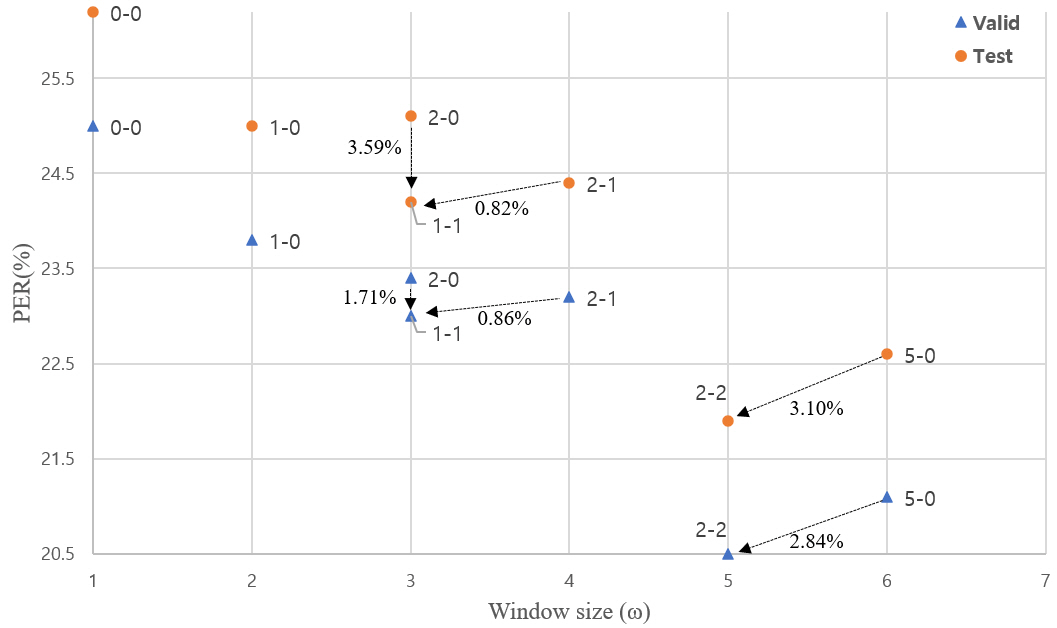
\includegraphics[width=0.5\linewidth]{04a_window_size.jpg}
\label{fig:diagram_win1}
}
\qquad
\subfloat[rcontext][PERs by expanding the size of the balanced window slices]{
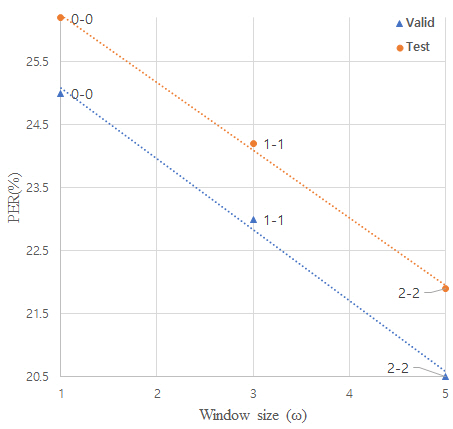
\includegraphics[width=0.35\linewidth]{04b_window_rcontext.jpg}
\label{fig:diagram_win2}
}
\caption[]{Phoneme error rates (PERs) depending on the configuration of window contexts)}
\label{fig:diagram_window}
\end{figure}

In order to observe the changes in accuracy depending on the configurations related to $\omega$, we compared 7 models as shown in Table~\ref{Tab:window}.
With the consideration of algorithmic delay caused by the right context size of windows $\omega_R$, all models have longer or equal left context size $\omega_L$ to their $\omega_R$.
As $\omega$ is expanded from 1 to 6, the numbers of required parameters (Params.) are increased from 0.21 to 0.66 million (M) as explained in  Section 3.2.
The RPERRs are at most 18.0\% and 16.4\% for Valid and Test respectively depending on $\omega$ settings as shown in the table.
When both context sizes are set to two, the model shows the best performance with 0.9M less parameters compared to the case where the left context size is set to 5.
The relationship between $\omega$ (X-axis) and PERs (Y-axis) are more explicitly described in Fig.~\ref{fig:diagram_window}.
``2-1" indicates that $\omega_L$ and $\omega_R$ are 2 and 1 respectively and the exact figures of the corresponding PERs are in Table~\ref{Tab:window}.
Triangles and circles indicate Valid and Test respectively.
We can see multiple cases where the balance of $\omega_L$ and $\omega_R$ has more of an effect on lowering the PERs than the number of parameters when $\omega > 1$ in Fig.~\ref{fig:diagram_win1}.
This phenomenon is described by the dashed arrows in the figure and the percentages beside the arrows are RPERR between the balanced and unbalanced window configurations.
Moreover, PERs of the three evenly sliced cases, that are ``0-0", ``1-1", and ``2-2", show an almost linear error reduction according to their $\omega$ for both evaluation sets from 25.6\% to 21.2\% on average as shown in Fig~\ref{fig:diagram_win2}.

\begin{table}[]
\centering
\begin{tabular}{cccc}
\multirow{2}{*}{Depth} & Params. & \multicolumn{2}{c}{PER(\%)} \\ 
                       & (M)     & Valid & Test \\\hline
2 & 0.14 & 26.7 & 28.0 \\
4 & 0.19 & 24.1 & 25.2 \\
8 & 0.39 & 23.0 & 24.2 \\
16 & 1.15 & 20.8 & 22.1
\end{tabular}
\caption{Phoneme error rates (PERs) depending on the depth of capsule groups}%
\label{Tab:depth}
\end{table}

We also performed experiments on the capsule group depth, by doubling it continually from 2 to 16, to examine its effect as in Table~\ref{Tab:depth}.
In these experiments, $\omega_L$ and $\omega_R$ are fixed to 1.
As capsule group depths increased, the required Params. are also increased nearly proportional to the depths from 0.14M to 1.15M as explained in Section 3.2.
The RPERRs for Valid and Test are 22.10\% and 21.07\% respectively.
The PER reductions slow down at depth 4 from 2.6\% and 2.8\% to 1.1\% and 1.0\% for Valid and Test respectively, even though the parameter increase is 4 times larger from 0.5 to 2.

\begin{table}[ht!]
\begin{tabular}{c|ccc|c}
\multirow{2}{*}{Model} & Online   & Params. & \multicolumn{2}{c}{PER(\%)} \\
                       & Decoding & (M)     & Valid & Test \\\hline
BLSTM-5L-250H~\citep{DBLP:conf/icassp/GravesMH13} & X& 6.80 & - & 18.4 \\
ULSTM-3L-421H~\citep{DBLP:conf/icassp/GravesMH13} & O& 3.80 & - & 19.6 \\
CNN-10L-maxout~\citep{DBLP:conf/interspeech/ZhangPBZLBC16} & O & 4.30 & 16.7 & 18.2 \\
RNN-T-3L-250H~\citep{DBLP:conf/icassp/GravesMH13} & X& 4.30 & - & 17.7 \\\hline
TF-5L  & X & 1.99 & 19.4 & 20.0 \\
TF-10L & X & 3.63 & 17.6 & 18.8 \\
TF-20L & X & 6.93 & 17.1 & 18.4 \\\hline
SRF-1L & O & 1.01 & 20.2 & 21.5 \\
SRF-2L & O & 0.99 & 19.2 & 21.3 \\
SRF-5L & O & 1.58 & 16.7 & 18.4 \\
SRF-7L & O & 1.97 & 16.0 & 17.4 \\
\end{tabular}
\caption{Phoneme error rates (PERs) comparisons depending on model structures}
\label{Tab:pc}
\end{table}

We compared the SRF models with the other CTC networks and RNN-T networks by stacking up the capsule layers which are made of the configurations, $P_H=60$, $C_H=30$ and $\omega=3$ $(\omega_L=1, \omega_R=1)$, as shown in Table~\ref{Tab:pc}.
The BLSTM-based CTC network, which consists of 5 bi-directional layers of 250 LSTM cells (BLSTM-5L-250H), shows 1.2\% better PRR for Test than its stream enabled version which is made of three uni-directional layers of 421 LSTM cells (ULSTM-3L-421H)~\citep{DBLP:conf/icassp/GravesMH13}.
CNN-10L-maxout~\citep{DBLP:conf/interspeech/ZhangPBZLBC16}, consists of 10 convolutional layers using maxout plus 1 max pooling layer after the first convolutional layer and is followed by three fully-connected layers activated by maxout.
The network shows the best accuracy in PRR among the compared CTC networks at 83.3\% and 81.8\% on Valid and Test respectively.
The RNN-T network (RNN-T-3L-250H)~\citep{DBLP:conf/icassp/GravesMH13} consists of a pre-trained CTC network, which is composed of 3 bi-directional layers of 250 LSTM cells, and an additional hidden layer of 250 LSTM cells as a prediction network.
RNN-T-3L-250H shows the best PRR of 82.3\% with 4.3M parameters.
We also performed the evaluations using Speech-Transformer~\citep{8462506}-based CTC networks which we implemented.
Convolutional layers in front of Transformer encoders have the same structures with the first sub-block of the capsulation block as explained in Section 4.1.2.
In each layer, $d_{emb}$ is set to 128 and the dimension of position-wise fully connected feed-forward layers is set to 1024. 
When it comes to learning rate decay, $\kappa$ is set to 1.5 and reduced to 0.5 under the same condition as the cases of the CapsNets and $n_{w}$ is set to 1,000.
The number of attention headers is set to 4 and there are approximately 15,250 frames in a batch according to the length of utterances.
In order to prevent overfitting, we set dropout rates for the input data, attention header, inner layers and residual connection to 0.3, 0.3, 0.4, and 0.4 respectively.
The other configurations are the same as explained in Section 4.1.2.
We added bigger penalties to non-diagonal elements in attention maps before applying the softmax function Eq.~\ref{eq:softmax}, depending on the distance $\delta$ from the diagonal of the maps in the form of $-\log(1+\delta \times \beta)$ as described in~\citep{8462506}, where $\beta$ is a scaling factor and we set this to 1.0.
TF-5L indicates that the Transformer consists of 5 encoder layers. The model consists of a similar number of parameters as the biggest SRF model at the bottom of the table.
Although the model shows the lowest accuracy among the comparison models, it is easily improved by stacking the encoder layers.
We compared 2 more Transformer-based CTC networks on Test with the LSTMs-based networks composed of a similar number of parameters.
The Transformer model consisting of 10 layers shows 4.08\% of RPERR with 0.17M less parameters compared to the ULSTM-based CTC network which has online decoding capability.
TF-20L shows the same PER compared to the corresponding BLSTM-based CTC network with slightly (0.13M) more parameters.

The reason why SRF-1L requires 0.02M more parameters than SRF-2L is that SRF-1L directly connects primary capsule groups to class capsule groups thus SRF-1L needs 11,340 (60 $\times$ 63 $\times$ 3) transform matrices while SRF-2L needs 11,040 ((60 $\times$ 30 + 30 $\times$ 63) $\times$ 3) transform matrices.
When comparing the two models, the number of capsule layers seems to have more of an effect on improving the accuracy than the number of parameters as in Table~\ref{Tab:pc}.
With 5 layers (SRF-5L), the model shows similar accuracy to the BLSTM-based CTC network while requiring 76.8\% less parameters.
By adding more layers, the proposed method finally attains 17.4\% of PER with the model consisting of 7 capsule layers (SRF-7L) for Test.
It is 2.2\% more accurate than ULSTM-3L-421H, which is the online capable version of LSTM, and 0.8\% better PRR compared to CNN-based structure.
Even more, the PER of SRF is slightly lower (RPERR is 1.65\%) than that of RNN-T-3L-250H while keeping online decoding capability. 
Lastly, SRF requires 45.8\% of parameters compared to both the CNN-based CTC network and the RNN-T.

\section{Analysis}
\begin{figure*}[ht!]
  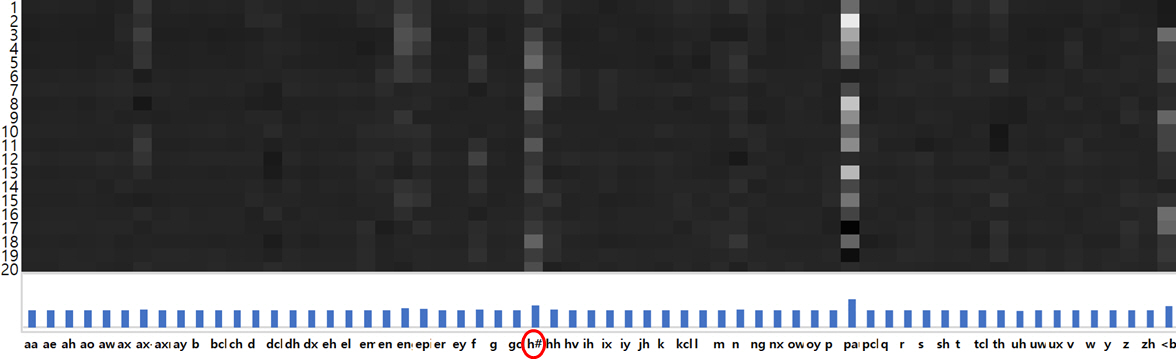
\includegraphics[trim={0 0cm 0 0cm}, clip, width=1.0 \linewidth]{05_coupling_coefficient_map.jpg}
  \caption{A heat map of coupling coefficients $c$ (SDR, Iteration=1, $t$=137)}
  \label{fig:cc}
\end{figure*}
In this section, we investigate how the routing method works in SRF by observing the heat maps of $c$ for a 5.47 seconds length utterance in the test set.
In the heat maps, brighter cells refer to larger values ranging from 0.01 to 0.05.
All models explained in this section are the same as explained in Table~\ref{Tab:iter} of Section 4.2.
Fig.~\ref{fig:cc} is a heat map of $c$ which maps from primary capsules (vertical axis) to class capsules (horizontal axis) of the iteration 1 version of the SDR model at $t=137$.
A corresponding reference label is the red circled symbol ``h\#”, which indicates the end of a sentence.
The numbers on the vertical axis indicates primary capsule indexes.
The bar graphs at the bottom of the figure represents the summation of coefficients per each class capsule.
The summation of each row, i.e. the summation of coefficients per each primary capsule, is one and the coefficients which route capsules to the padding symbol are masked to zero as explained in Section 3.2 and they are not represented in the heat map.
As shown in the figure, primary capsules are mostly routed to a class capsule corresponding to a ``pau” symbol with the accumulated coefficient of 0.52 then followed by ``h\#" with that of 0.41 and ``$<$blank$>$" with that of 0.39.
7 primary capsules indexed by in the order of 17, 19, 20, 6, 7, 12 and 5 are routed more to the class capsule corresponding to the correct symbol ``h\#" rather than the capsule for ``pau".

\begin{figure*}[ht!]
  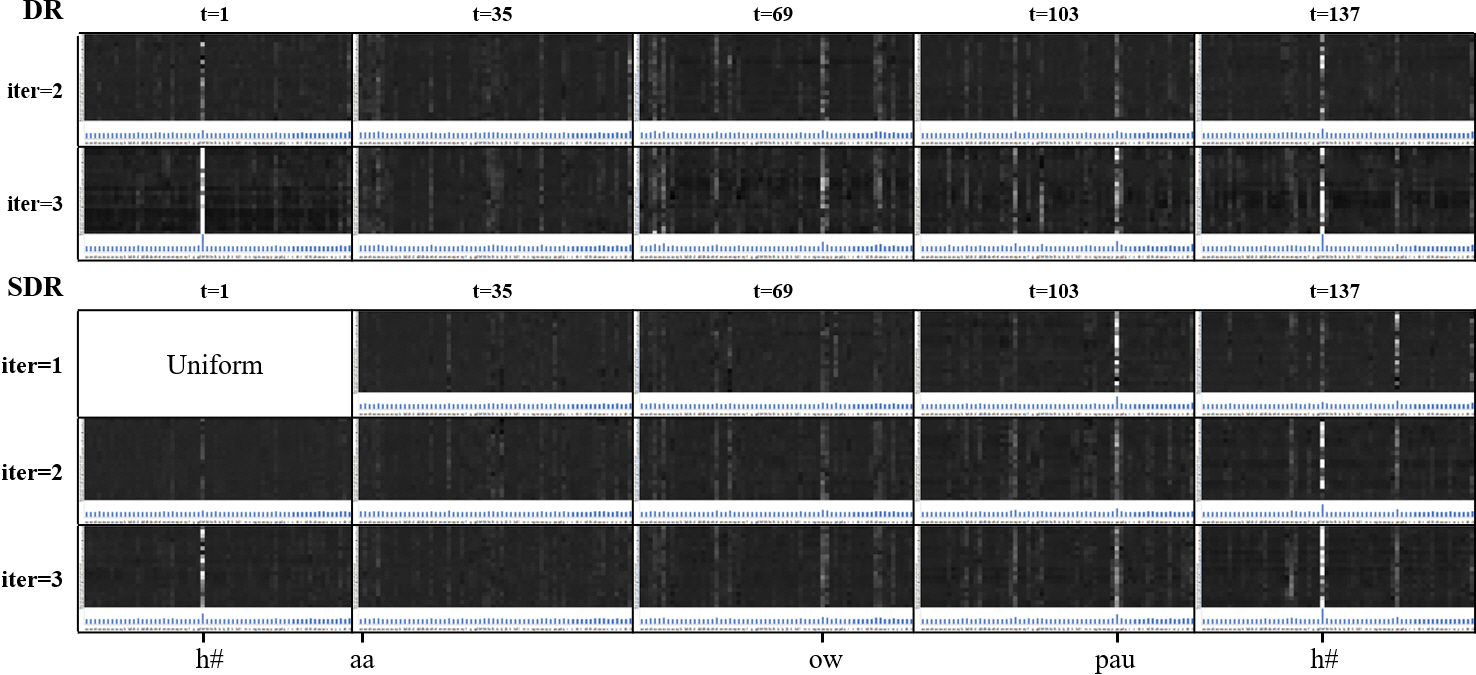
\includegraphics[trim={0 0cm 0 0cm}, clip, width=1.0 \linewidth]{06_coupling_coefficient_maps.jpg}
  \caption{Heat maps of coupling coefficients $c$ for DR and SDR}
  \label{fig:ccm}
\end{figure*}
We compare 14 heat maps for different iteration numbers from 1 to 3 between DR and SDR as in Fig.~\ref{fig:ccm}.
The coefficients of iteration 1 version of DR are all the same so it is not included in the figure.
The reference symbols for each $t$ are written in the bottom of the figure with the time markers.
The majority of primary capsules are routed to the class capsule corresponding to the correct symbol.
Among the two DR cases, the heat maps of the iteration 3 versions have a slightly higher contrast than that of the iteration 2 versions as shown in Fig.~\ref{fig:ccm}.
In order words, as the number of iterations increases, it seems that the distributions become less uniform.
The iteration 2 and 3 version of SDR models display the same phenomenon as the DR version.
However, the SDR model with iteration 1 seems to have different behaviors besides that $c$ is uniform at $t=1$.
The model routes the capsules to ``pau" more than any other version at $t=103$.
Moreover, at $t=137$, i.e. the end of the sentence, the model seems to route the majority of capsules to the class capsules corresponding to ``pau" rather than the correct symbol ``h\#" as explained earlier in this section.

\begin{figure*}[ht]
\centering
\subfloat[size][$t$: 1 $\to$ 10]{
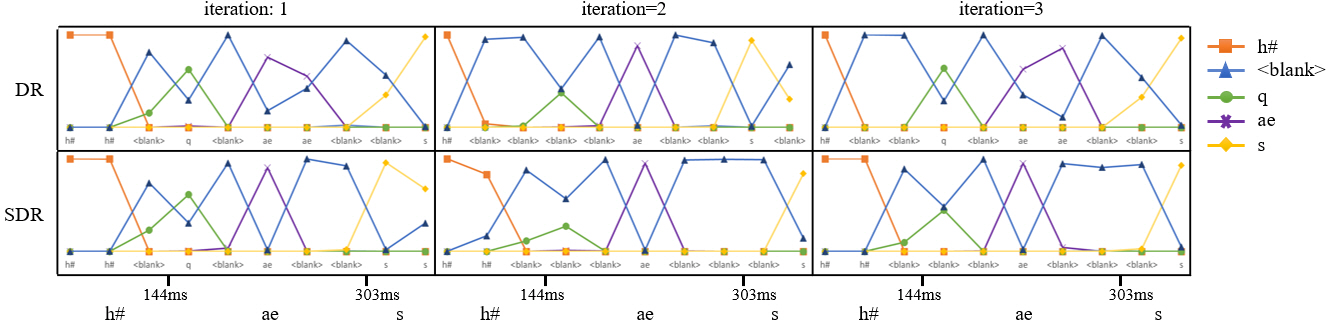
\includegraphics[width=1.0\linewidth]{07a_softmax_output_start.jpg}
\label{fig:softmax_start}
}
\qquad
\subfloat[size][$t$: 127 $\to$ 137]{
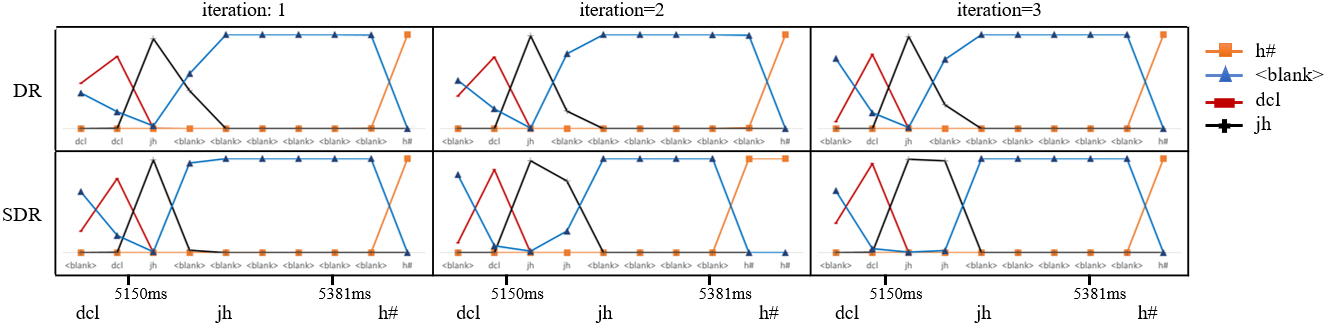
\includegraphics[width=1.0\linewidth]{07b_softmax_output_end.jpg}
\label{fig:softmax_end}
}
\caption[]{Softmax vectors depending on routing methods (X-axis: time (ms), Y-axis: probability)}
\label{fig:softmax_output}
\end{figure*}

In order to see how the phenomenon affects alignment, we checked the 10 probability vectors each at the beginning and end of the sentence as shown in Fig~\ref{fig:softmax_output}.
Symbols are represented with different line shapes described in the right side of the figure.
The labels on the X-axis of each graph indicate a symbol with the highest probability, i.e. the phoneme sequence of the greedy decoding.
Reference time markers and symbols are written at the bottom of Fig~\ref{fig:softmax_start} and Fig~\ref{fig:softmax_end}.
For all the cases, no phenomenon of misalignment of the iteration 1 version of SDR model is observed.
It is not a big difference, but rather, the SDR model recognizes the symbol ``s" as fast as the iteration 2 version DR as shown in Fig~\ref{fig:softmax_start}.
The end of sentence symbol ``h\#" is also precisely recognized in all the cases as in Fig~\ref{fig:softmax_end}.
Even in the case of SDR when iteration is set to 1 at $t=137$, unlike the heat map which routes most of the primary capsules to the class capsule to the symbol ``pau", the probability of ``h\#" is the largest.

\section{Related work}
In this paper, we explored the potential capabilities of CapsNets for sequence encoding.
There have been many research related to CapsNets such as improving their routing mechanisms or applying them to various kinds of tasks.
In this section, we explain those attempts.
The concept of routing between capsules was first introduced to recognize pose information~\citep{DBLP:conf/icann/HintonKW11} and it was implemented in an auto encoder manner~\citep{DBLP:conf/nips/HintonZ93}.
DR~\citep{DBLP:conf/nips/SabourFH17} is the earliest attempt to apply capsules for image classification problems. It showed better accuracy, not only in the original MNIST~\citep{lecun-mnisthandwrittendigit-2010} dataset compared to CNNs, but also in highly overlapping digit cases in the MultiMNIST dataset.
The accuracy on the overlapping cases was on par with that of sequential attention models.
EM routing~\citep{DBLP:conf/iclr/HintonSF18} is a follow-up study of DR.
It not only releases the length constraint of the instantiation vectors by defining activations as separate scalars but also reduces the size of transformation matrices to the square root size by representing the instantiation parameters as matrices.
In addition, an expectation-maximization (EM) algorithm based on the Gaussian mixture model is applied to the routing method.
Despite its structural and theoretical advances, the EM routing method has shown noncompetitive accuracy and computational complexity compared to DR~\citep{Malmgren1314210, DBLP:conf/nips/HahnPK19}.
This is the reason why we did not adopt it in this study, but it still has a suitable structure to be applied to the proposed method.

In order to improve implementations of the pioneer studies, various modifications were proposed.
When it comes to iterative routing methods, since increasing the number of iterations can lead to unbalanced activations, ~\citep{DBLP:conf/iclr/Wang018} proposed an optimized DR method which applies an entropy regularizer to constrain the routing coefficient to be close to the uniform distribution.
A min-max normalization~\citep{DBLP:journals/corr/abs-1903-09662} was applied to resolve the performance degradation in DR caused by iterative usage of a softmax function as a normalization function for routing coefficients. 
For faster training, routing coefficients were initialized from the learnable weights~\citep{DBLP:conf/eccv/RamasingheAK18} and an attempt to introduce the EM algorithm to DR~\citep{DBLP:series/sci/Zhang0W19} under certain conditions was studied.
Recently, CapsNet has been applied to relatively large datasets such as CiFAR 100~\citep{Krizhevsky09learningmultiple} by parallelizing iterative routing methods~\citep{DBLP:conf/iclr/TsaiSGS20} and showed competitive performance compared to ResNet~\citep{DBLP:conf/cvpr/HeZRS16}.
There is also self-routing~\citep{DBLP:conf/nips/HahnPK19}, which is a non-iterative routing method, that introduces the mixture-of-expect mechanism~\citep{DBLP:journals/neco/JacobsJNH91} to the routing method.

In addition to research which improves CapsNets themselves, there are various attempts to merge CapsNets or the routing mechanism with other models.
Especially for sequence inputs, CapsNets are combined with existing sequential models either as a successor block at the top of the LSTM layers~\citep{zhang-etal-2018-attention, DBLP:conf/icann/HePLHZ19}, the Transformer~\citep{DBLP:conf/nips/VaswaniSPUJGKP17} encoder blocks~\citep{liu-etal-2019-transformer}, and bidirectional encoder representations from Transformers (BERT)
~\citep{DBLP:conf/naacl/DevlinCLT19, DBLP:journals/jbi/SunYWZLW20} or as an intermediate block in between encoders and decoders which are made of LSTMs~\citep{wang-2019-towards}.
There are also attempts to put routing algorithms into attention methods and vice versa.
Routing mechanisms are adopted into self-attention based models to cluster similar information from the multi-head attentions~\citep{DBLP:conf/nlpcc/GuF19}.
In contrast, STAR-Caps~\citep{DBLP:conf/nips/AhmedT19} merges attention methods into the routing mechanism.

CapsNets have been actively applied to a variety of fields because of their outstanding image encoding abilities.
They are suitable for visual tracking~\citep{DBLP:journals/corr/abs-1902-10054} and object segmentation of medical images~\citep{DBLP:journals/corr/abs-1804-04241}.
CapsNets also can be easily applied to non-visual tasks such as knowledge graph embedding and link prediction because of their representations of conceptual hierarchy relationships~\citep{DBLP:conf/naacl/NguyenVNNP19, DBLP:conf/iclr/XinyiC19}.
For linguistic data, CapsNets were applied to text classification with k-means routing~\citep{DBLP:journals/corr/abs-1810-09177}, machine translation in an encoder-decoder manner~\citep{wang-2019-towards}, user intent detection~\citep{DBLP:conf/emnlp/XiaZYCY18, DBLP:conf/acl/ZhangLDFY19} and emotion detection using micro blogs~\citep{DBLP:journals/nca/ZhongLLCLDWZ20}.
Classification tasks using audio and speech data~\citep{DBLP:journals/corr/abs-1902-05069} have also been actively researched to detect sound events~\citep{DBLP:conf/eusipco/Iqbal0KW18, DBLP:journals/jstsp/VesperiniGPS19} and classify emotions~\citep{DBLP:conf/icassp/WuLCLYDMHWLM19}.
Electrocardiogram signal categorization~\citep{Jayasekara2019TimeCapsCT} is another interesting task where CapsNets can be applied to classify input sequential data.
Last but not least, isolated word recognition has been researched~\citep{DBLP:conf/interspeech/BaeK18, xiongyan2018master}.

\section{Conclusion}
In this study, we proposed SRF, which is a novel framework to adapt CapsNets for encoding sequence data.
We believe, this is the first capsule-only structure for seq2seq recognition.
In the framework, input sequences are capsulized and sliced by the given window size.
Routing from lower to higher levels is performed for each window slice by temporally sharing two kinds of parameters over a whole sequence.
From the perspective of gradient-based optimization, the amount of required memory size can be controlled regardless of the length of input sequences by sharing the transformation matrix.
Moreover, by initializing routing coefficients based on the routing output of the previous window slices, we could minimize decoding speed degradation caused by the routing iteration since the routing mechanism can be operated in a non-iterative manner during inference.
The proposed method achieved competitive performance on a phoneme recognition task compared to CNNs, LSTMs, and Transformers in three aspects that are accuracy, amount of required memory, and streaming capabilities.
An area of improvement for the future is the possibility of a fully end-to-end ASR system, which can represent linguistic context, based on CapsNet only architectures.

\bibliography{mybibfile}

\end{document}
